\section{Festkonzept}

\subsection{Allgemein}


\begin{frame}[c]{Übersicht Festkonzept}
    \begin{itemize}
        \item Keine Floors
        \item Drei Bühnen:
            \begin{itemize}
                \item Forumsbühne (Mainstage am Forum)
                \item Karlsruher Bühne (Paulckeplatz)
                \item DJ Bühne (Otto-Amann-Platz)
            \end{itemize}
        \item Umzäuntes Gelände, Tickets für 5\EUR/Tag
        % \item (Aufbau-) Helfer bekommen Tickets erstattet (für den Tag an dem sie Helfen)
        \item Helfer bekommen gratis Eintritt für den Tag, an dem sie helfen
    \end{itemize}
\end{frame}


\subsection{Update Geländeplan}

\begin{frame}[c]{Geländeplan}
    % trim = l b r t
    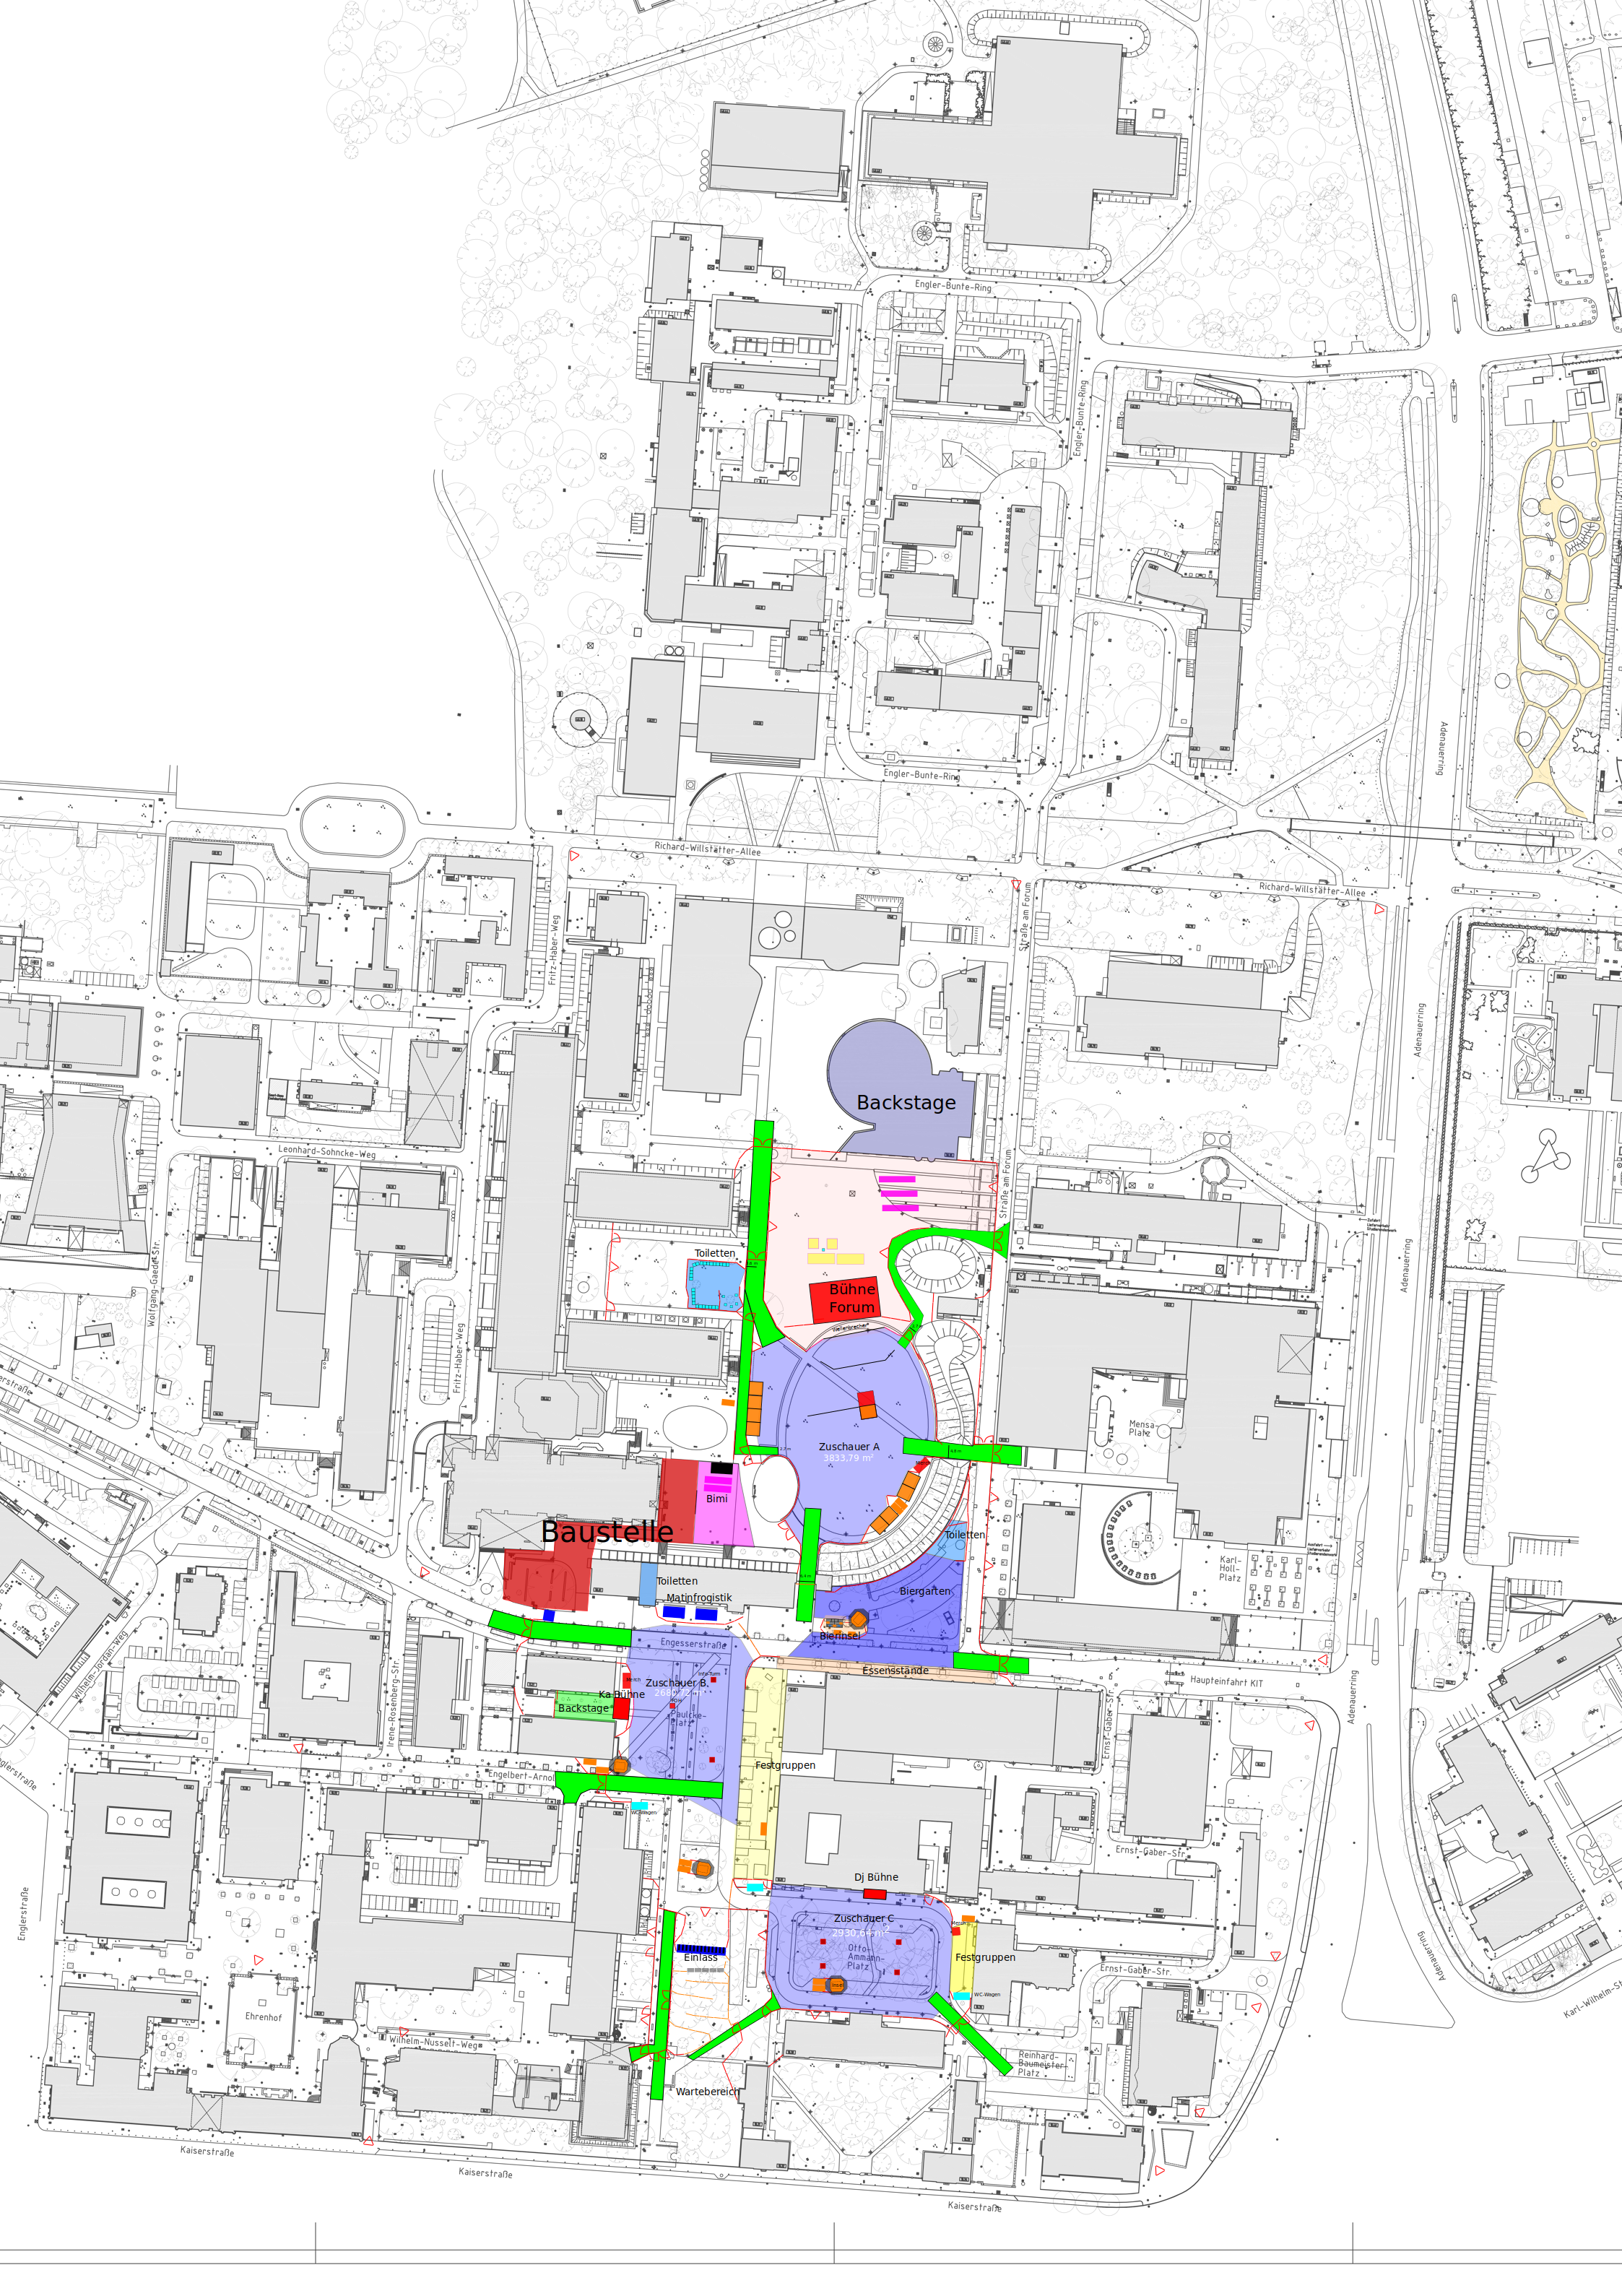
\includegraphics[height=0.95\textheight,clip,trim = 500 150 700 1400]{Plan_Freitag}
\end{frame}




\subsection{Auf- und Abbau}

\begin{frame}[c]{Unser Vertrag mit euch}
    \begin{itemize}[<+(1)->]
        \item Wir stellen euch Materialien für einen Stand
        \item Dafür helft ihr beim Auf- und Abbau des gesamten Fests
        \item<handout> Euren Stand als auch Allgemein, sonst kann das UniFest nicht stattfinden
        \item<handout> Insbesondere erwarten wir von euch, dass Ihr Abbauhelfer stellt
    \end{itemize}
    \Large
    \pause
    Dann wird das ein EPISCHES UNIFEST!
\end{frame}


\begin{frame}[c]{Deadlines Aufbau}
    \begin{itemize}[<+(1)->]
        % \item Dienstag werden die Zelte im Forum aufgestellt
        \item Die Zelte im \textbf{Forum} werden \textbf{Dienstag} aufgebaut
        \item Stände am \textbf{Paulcke}-Platz müssen bis \textbf{Mittwoch 16 Uhr} aufgebaut sein
        \item Mittwochabends wird am Paulcke-Platz Programm sein
        \item Stände am \textbf{Otto-Amann}-Platz müssen bis \textbf{Mittwoch 22 Uhr} aufgebaut sein
        \item Donnerstag wird Programm am Otto-Amann-Platz sein
    \end{itemize}
\end{frame}


\begin{frame}[c]{Schichten für Auf- und Abbau}
    \begin{itemize}[<+(1)->]
        \item Täglich 9-13 Uhr und 14-18 Uhr
        \item<handout> Sowie bei Bedarf 19-23 Uhr
        \item Aufbau fängt ab Montag (davor) an
        \item Abbau läuft bis Dienstag (danach)
        \item Angemessene Verpflegung für Helfer
        \item<handout> Ihr könnt auch außerhalb von Schichten helfen!
    \end{itemize}
\end{frame}



\subsection{Helfersystem}

\begin{frame}[c]{Helfersystem}
    \begin{itemize}[<+(1)->]
        \item Wir arbeiten dieses Jahr mit einem neuen Helfersystem
        \item Es soll die Arbeit für alle einfacher machen
        \item Wir geben euch noch eine detaillierte Einführung!
        \item<handout> Vermutlich beim nächsten Treffen
    \end{itemize}
\end{frame}


